\chapter{كيمياء الحالة الصلبة: الحزم والعيوب وأشباه الموصلات}\label{ch:b3:solid-state}

اللوح الشمسي على السطح والصمام الثنائي الباعث للضوء في المصباح مصنوعان من
الصنف نفسه من البلورات، السيليكون أو مركب للغاليوم مع النيتروجين أو الزرنيخ
أو الفوسفور، أُدخلت فيه عمدًا بضع ذرات شائبة في كل مليون. ويحدد
عملهما أمران لا يملكهما الجزيء: حزم من
مستويات الطاقة، مع فجوة يحدد عرضها الضوء الذي تمتصه البلورة أو
تصدره، والعيوب، التي تحمل الشحنات. ويبني هذا الفصل الحزم
من المدارات الجزيئية، ويعدّ حاملات الشحنة في \omterm{def:b3:solid-state:classes}{شبه موصل}، ويعامل
الذرات المفقودة والمنزاحة عن مواضعها على أنها أنواع كيميائية لها توازناتها الخاصة،
وصولًا إلى \omterm{def:b3:solid-state:ionic-conductor}{الإلكتروليت الصلب} في مستشعر الأكسجين في عادم السيارة.

\begin{recall}
عرّف مجلد السنة الأولى البلورات، والرابطة الفلزية، والبلورات الأيونية 
والتساهمية، والمواقع الخلالية والسبائك، ومعادلة نرنست؛ وعرّف مجلد السنة الثانية
طريقة هوكل وتكامل الرنين $\beta$.
وأعطى \cref{ch:b3:x-ray-diffraction} \omterm{def:b3:x-ray-diffraction:reciprocal}{الشبكة المقلوبة}، 
و\cref{ch:b3:partition-functions} \omterm{def:b3:partition-functions:boltzmann}{توزيع بولتزمان} 
\omterm{def:b3:partition-functions:statistical-entropy}{والإنتروبيا الإحصائية} $S = k\ln W$.
\end{recall}

\begin{omfigure}
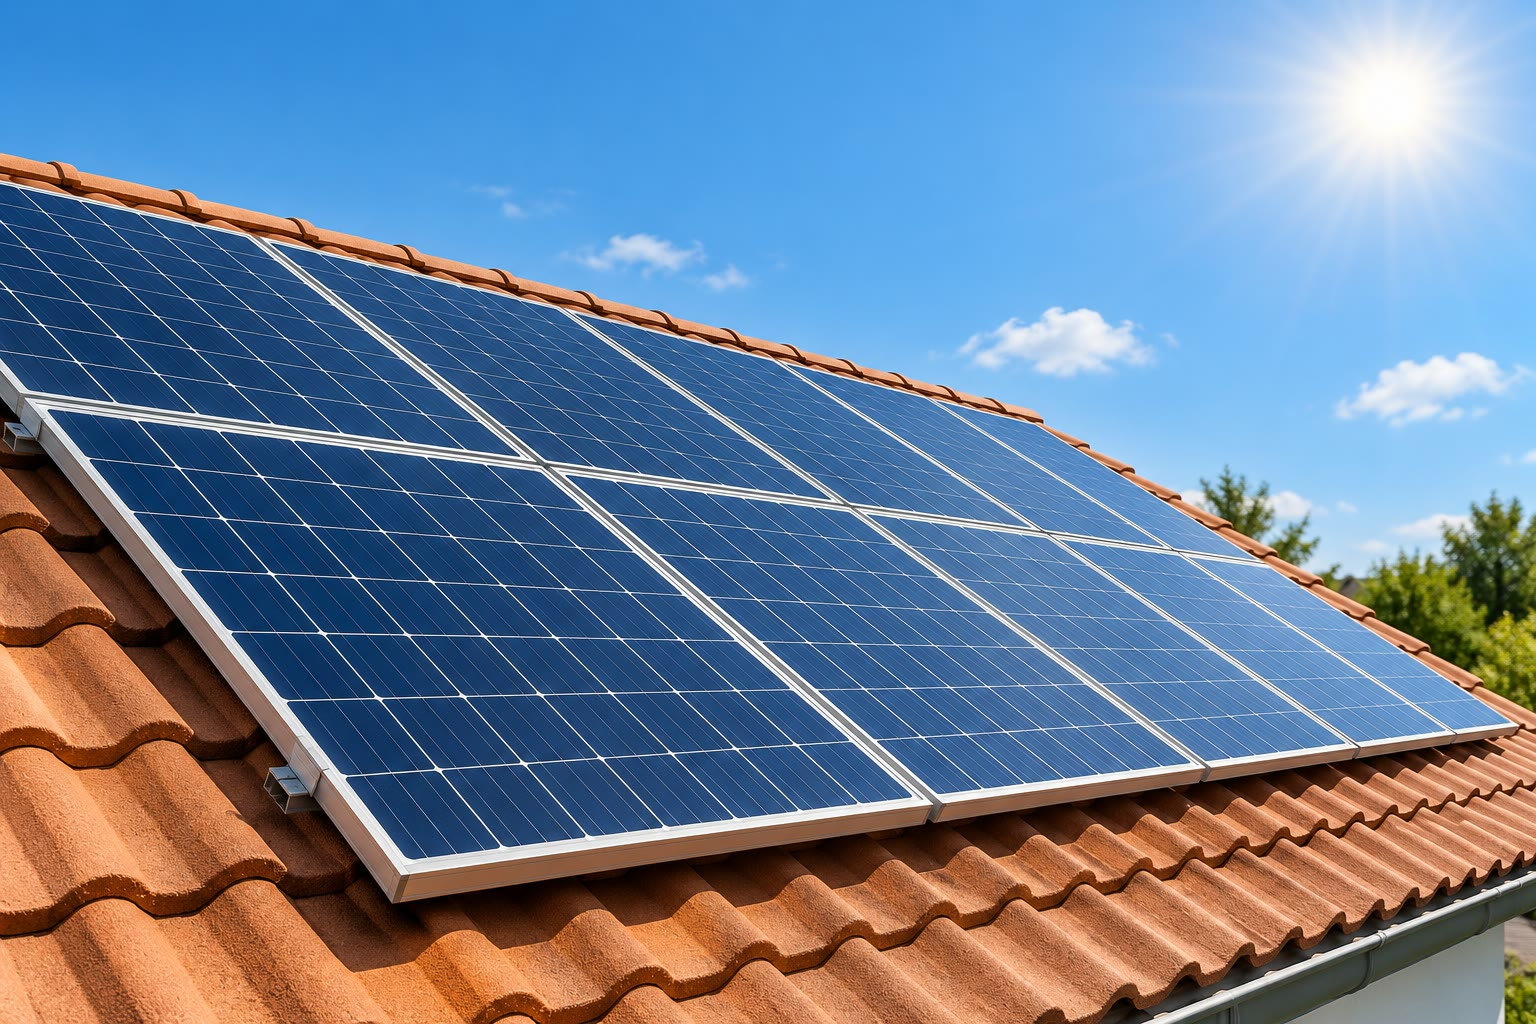
\includegraphics[width=0.6\linewidth]{images/book4/ai/b3-22-solar-panels.jpg}

{\small ألواح شمسية على سطح مكسو بالقرميد: كل خلية شريحة رقيقة من السيليكون
يرفع فيها الضوء الإلكترونات عبر \omterm{def:b3:solid-state:band}{فجوة حزمية} تبلغ نحو إلكترون فولت واحد.}
\end{omfigure}

\section{من المدارات إلى الحزم}

لنأخذ سلسلة من $N$ ذرة متماثلة، لكل منها مدار s واحد، في تقريب
هوكل: تكامل كولوم $\alpha$ على كل ذرة، وتكامل الرنين $\beta < 0$
بين الجارتين، وصفر فيما عدا ذلك.

\begin{theorem}[مستويات سلسلة هوكل]\label{thm:b3:solid-state:chain}
للمدارات الجزيئية $N$ لسلسلة خطية من $N$ ذرة الطاقات
\[
  E_k = \alpha + 2\beta\cos\frac{k\pi}{N + 1}, \qquad k = 1, \dots, N,
\]
مع المعاملات $c_j^{(k)} \propto \sin\bigl(jk\pi/(N + 1)\bigr)$ على الذرة $j$. وحين $N \to \infty$ تملأ المستويات
المجال من $\alpha + 2\beta$ إلى $\alpha - 2\beta$ ملئًا كثيفًا: أي حزمة عرضها $4|\beta|$.
\end{theorem}

\begin{proof}
المعادلات القرنية هي $\beta c_{j-1} + (\alpha - E)c_j + \beta c_{j+1} = 0$ من أجل $j = 1, \dots, N$، مع $c_0 = c_{N+1} = 0$
(لا ذرة هناك). لنجرّب $c_j = \sin(j\theta)$: لما كان $\sin((j - 1)\theta) + \sin((j + 1)\theta) = 2\cos\theta\sin(j\theta)$، تصير كل
معادلة $(\alpha - E + 2\beta\cos\theta)\sin(j\theta) = 0$، ومنه $E = \alpha + 2\beta\cos\theta$. والشرط $c_0 = 0$ محقق
لكل $\theta$، و$c_{N+1} = \sin((N + 1)\theta) = 0$ يقتضي $\theta = k\pi/(N + 1)$؛ و$k = 1, \dots, N$ تعطي $N$ مستوى
متمايزًا (والقيم الأخرى تكررها أو تنعدم). والأدنى والأعلى هما
$\alpha \pm 2\beta\cos(\pi/(N + 1))$، اللذان يؤولان إلى $\alpha \pm 2\beta$؛ والمسافة بين مستويين متجاورين لا تتجاوز
$2|\beta|\pi/(N + 1)$، التي تؤول إلى الصفر.
\end{proof}

من أجل $N = 2$ تعطي المبرهنة $\alpha \pm \beta$، أي مدارات النظام $\pi$ في الإيثين؛ ومن أجل
$N = 6$ الهكساترايين المفتوح السلسلة. وفي الأبعاد الثلاثة يحدث الأمر نفسه مع
كل أنواع المدارات الذرية: فالمدارات s تعطي حزمة s، والمدارات p حزمة p،
وكل حزمة تتسع لعدد $2N$ من الإلكترونات من أجل $N$ ذرة.

\begin{definition}[الحزم]\label{def:b3:solid-state:band}
\emph{حزمة الطاقة}\index{حزمة الطاقة} في بلورة مجال متصل من
طاقات الإلكترون الواحد المسموح بها، يتكوّن من مدارات كل ذراتها. 
و\emph{الفجوة الحزمية}\index{فجوة حزمية} $E_g$ مجال من الطاقات لا مستويات فيه بين
حزمتين. وفي \omterm{def:b3:solid-state:classes}{شبه الموصل} أو \omterm{def:b3:solid-state:classes}{العازل} عند درجة الصفر المطلق، تسمى أعلى
حزمة ممتلئة \emph{حزمة التكافؤ}\index{حزمة التكافؤ} وأدنى حزمة فارغة
\emph{حزمة التوصيل}\index{حزمة التوصيل}.
\end{definition}

\begin{definition}[كثافة الحالات ومستوى فيرمي]\label{def:b3:solid-state:fermi}
\emph{كثافة الحالات}\index{كثافة الحالات} $g(E)$ هي عدد
المستويات لوحدة الطاقة (ولكل ذرة أو لوحدة الحجم) قرب الطاقة $E$.
و\emph{مستوى فيرمي}\index{مستوى فيرمي} $E_F$ هو الطاقة التي يكون عندها
احتمال \omterm{def:b3:partition-functions:boltzmann}{إشغال} المستوى $1/2$؛ وعند الصفر المطلق تكون كل المستويات التي تحته
ممتلئة وكل التي فوقه فارغة.
\end{definition}

\begin{omfigure}
\begin{tikzpicture}
\begin{axis}[width=0.78\linewidth, height=6.2cm, xmin=0.3, xmax=7.6, ymin=-2.3, ymax=2.3,
  axis lines=left, xtick={1,2,3,4,5,6.6}, xticklabels={2,4,8,16,64,$\infty$: $g(E)$},
  xlabel={\foreignlanguage{arabic}{عدد الذرات $N$}}, ylabel={$(E - \alpha)/|\beta|$},
  ytick={-2,-1,0,1,2}, tick label style={font=\small}, label style={font=\small}]
\addplot[only marks, mark=-, mark size=7pt, omDef, thick] table[x=col, y=e] {figdata/out/bachelor-3-band-chain.dat};
\addplot[omThm, thick] table[x expr=6.0+0.55*\thisrow{g}, y=e] {figdata/out/bachelor-3-band-chain-b.dat};
\draw[black!40, dashed] (axis cs:0.3,-2) -- (axis cs:7.6,-2);
\draw[black!40, dashed] (axis cs:0.3,2) -- (axis cs:7.6,2);
\draw[<->, black!60] (axis cs:5.6,-2) -- (axis cs:5.6,2) node[midway, left, font=\scriptsize] {$4|\beta|$};
\end{axis}
\end{tikzpicture}

{\small مستويات هوكل لسلاسل من 2 إلى 64 ذرة (خط قصير لكل مستوى؛
ومع $\beta < 0$ تكون المستويات الرابطة في الأسفل). تتزاحم المستويات في حزمة
بين $\alpha + 2\beta$ و$\alpha - 2\beta$؛ وعلى اليمين، \omterm{def:b3:solid-state:fermi}{كثافة الحالات} للسلسلة
اللانهائية، وهي أكبر ما تكون عند حافتي الحزمة.}
\end{omfigure}

\begin{proposition}[ملء الحزم]\label{prop:b3:solid-state:filling}
البلورة التي تكون أعلى حزمها المشغولة مملوءة جزئيًا توصل الكهرباء
كالفلز؛ أما البلورة التي تكون حزمها إما ممتلئة وإما فارغة، مع فجوة
بينها، فلا توصل عند الصفر المطلق.
\end{proposition}

\begin{proof}[تعليل]
في مجال كهربائي، تكتسب الإلكترونات قليلًا من الطاقة والزخم: فيجب أن
تنتقل إلى مستويات فارغة فوق تلك التي تشغلها مباشرة. وفي حزمة مملوءة جزئيًا
تقع هذه المستويات فوق \omterm{def:b3:solid-state:fermi}{مستوى فيرمي} مباشرة، دون كلفة طاقية. أما في
الحزمة الممتلئة فكل مستوى مشغول والمستوى الفارغ التالي عبر الفجوة؛
فضلًا عن أن الحزمة الممتلئة لا تحمل تيارًا صافيًا، إذ يقابل كل إلكترون يتحرك
في اتجاه إلكترونٌ آخر يتحرك في الاتجاه المعاكس.
\end{proof}

الصوديوم، بإلكترون 3s واحد لكل ذرة، يملأ نصف حزمته s: فهو فلز.
والمغنيزيوم، بإلكترونين، كان سيملأ حزمته s تمامًا، لكن الحزمتين s وp
متداخلتان، فهو فلز أيضًا. وللألماس والسيليكون أربعة إلكترونات تكافؤ
لكل ذرة في مدارات تنشطر إلى حزمة رابطة ممتلئة وحزمة
مضادة للترابط فارغة، تفصلهما فجوة.

\begin{definition}[أشباه الموصلات والعوازل]\label{def:b3:solid-state:classes}
\emph{شبه الموصل}\index{شبه موصل} صلب له \omterm{def:b3:solid-state:band}{فجوة حزمية} صغيرة
بما يكفي (حتى نحو \qty{3}{eV}) لكي يعبرها عدد قابل للقياس من الإلكترونات
عند درجة الحرارة العادية أو بعد التطعيم؛ أما \emph{العازل}\index{عازل}
ففجوته كبيرة إلى حد أنه لا يوصل.
\end{definition}

\begin{omfigure}
\begin{tikzpicture}[font=\small]
  \foreach \x/\name in {0/{\foreignlanguage{arabic}{فلز}}, 3.6/{\foreignlanguage{arabic}{شبه موصل}}, 7.2/{\foreignlanguage{arabic}{عازل}}} {
    \node[font=\small\bfseries] at (\x+0.8,4.3) {\name};
  }
  % metal: one partly filled band
  \fill[omDef!55] (0,0.4) rectangle (1.6,2.0);
  \draw (0,0.4) rectangle (1.6,3.4);
  \draw[omThm, thick] (-0.25,2.0) -- (1.85,2.0) node[right, font=\scriptsize] {$E_F$};
  % semiconductor: small gap
  \fill[omDef!55] (3.6,0.4) rectangle (5.2,1.7);
  \draw (3.6,0.4) rectangle (5.2,1.7);
  \draw (3.6,2.5) rectangle (5.2,3.8);
  \draw[omThm, thick] (3.35,2.1) -- (5.45,2.1) node[right, font=\scriptsize] {$E_F$};
  \draw[<->] (4.4,1.7) -- (4.4,2.5) node[pos=0.8, right, font=\scriptsize] {$E_g$};
  % insulator: large gap
  \fill[omDef!55] (7.2,0.4) rectangle (8.8,1.2);
  \draw (7.2,0.4) rectangle (8.8,1.2);
  \draw (7.2,3.2) rectangle (8.8,4.0);
  \draw[omThm, thick] (6.95,2.2) -- (9.05,2.2) node[right, font=\scriptsize] {$E_F$};
  \draw[<->] (8.0,1.2) -- (8.0,3.2) node[pos=0.75, right, font=\scriptsize] {$E_g$};
  \node[font=\scriptsize, anchor=east] at (3.5,1.05) {\foreignlanguage{arabic}{التكافؤ}};
  \node[font=\scriptsize, anchor=east] at (3.5,3.15) {\foreignlanguage{arabic}{التوصيل}};
  \draw[->] (-0.6,0.2) -- (-0.6,3.9) node[above, font=\scriptsize] {$E$};
\end{tikzpicture}

{\small ملء الحزم عند الصفر المطلق (المستويات الممتلئة مظللة). للفلز
حزمة مملوءة جزئيًا \omterm{def:b3:solid-state:fermi}{ومستوى فيرمي} داخلها؛ ولشبه الموصل 
\omterm{def:b3:solid-state:classes}{والعازل} حزمة تكافؤ ممتلئة وحزمة توصيل فارغة، \omterm{def:b3:solid-state:fermi}{ومستوى فيرمي}
في الفجوة، الضيقة في الأول والواسعة في الثاني.}
\end{omfigure}

\section{أشباه الموصلات}

\begin{definition}[حاملات الشحنة]\label{def:b3:solid-state:carriers}
\emph{شبه الموصل الذاتي}\index{شبه موصل ذاتي} \omterm{def:b3:solid-state:classes}{شبه موصل}
نقي، تأتي كل حاملاته من إلكترونات مثارة عبر الفجوة. 
و\emph{حامل الشحنة}\index{حامل الشحنة} جسيم متحرك يحمل
التيار: إلكترون في \omterm{def:b3:solid-state:band}{حزمة التوصيل}، أو \emph{ثقب}\index{ثقب}، أي
مستوى فارغ في \omterm{def:b3:solid-state:band}{حزمة التكافؤ}، يتحرك كشحنة موجبة.
\end{definition}

\begin{theorem}[تركيز الحاملات الذاتي]\label{thm:b3:solid-state:intrinsic}
مع $N_c$ و$N_v$ الكثافتين الفعالتين للحالات في حزمتي التوصيل 
والتكافؤ (نقبلهما)، يكون تركيزا الإلكترونات \omterm{def:b3:solid-state:carriers}{والثقوب} في \omterm{def:b3:solid-state:classes}{شبه موصل}
يبعد \omterm{def:b3:solid-state:fermi}{مستوى فيرمي} فيه أكثر من بضعة $kT$ عن كل من حافتي الحزمتين
\[
  n = N_c\,\eu^{-(E_c - E_F)/kT}, \qquad p = N_v\,\eu^{-(E_F - E_v)/kT},
\]
وفي \omterm{def:b3:solid-state:carriers}{شبه موصل ذاتي}
\[
  n = p = n_i = \sqrt{N_cN_v}\,\eu^{-E_g/2kT}.
\]
\end{theorem}

\begin{proof}
\omterm{def:b3:partition-functions:boltzmann}{إشغال} مستوى طاقته $E$ هو $f(E) = 1/(1 + \eu^{(E - E_F)/kT})$. وحين
$E - E_F \gg kT$، $f \approx \eu^{-(E - E_F)/kT}$، أي ذيل بولتزمان. وبجمع هذا الذيل على كل مستويات \omterm{def:b3:solid-state:band}{حزمة
التوصيل} نحصل على $n = \int g_c(E)\eu^{-(E - E_F)/kT}\,\dd E = \eu^{-(E_c - E_F)/kT}\int g_c(E)\eu^{-(E - E_c)/kT}\,\dd E$، والتكامل الأخير هو بحكم
التعريف $N_c$. \omterm{def:b3:solid-state:carriers}{والثقوب} مستويات فارغة، احتمالها $1 - f \approx \eu^{-(E_F - E)/kT}$ في
\omterm{def:b3:solid-state:band}{حزمة التكافؤ}؛ والخطوات نفسها تعطي $p$. ثم $np = N_cN_v\eu^{-(E_c - E_v)/kT} = N_cN_v\eu^{-E_g/kT}$، وفي بلورة نقية
يترك كل إلكترون مثار ثقبًا واحدًا: $n = p$، ومنه $n = \sqrt{np}$.
\end{proof}

\begin{proposition}[قانون فعل الكتلة]\label{prop:b3:solid-state:mass-action}
في كل \omterm{def:b3:solid-state:classes}{شبه موصل} في حالة التوازن، مطعَّمًا كان أم لا، $np = n_i^2$.
\end{proposition}

\begin{proof}
الجداء $np = N_cN_v\eu^{-E_g/kT}$ الذي وجدناه في برهان
\cref{thm:b3:solid-state:intrinsic} لا يحوي $E_F$: فهو نفسه مهما كان ما
يحدد \omterm{def:b3:solid-state:fermi}{مستوى فيرمي}، ويساوي قيمته الذاتية $n_i^2$. وهو
ثابت توازن $\text{لا شيء} \rightleftharpoons \mathrm e^- + \mathrm h^+$، كالجداء الأيوني للماء.
\end{proof}

\begin{omfigure}
% ledger: eg:Si.E0, eg:Si.a, eg:Si.b, eg:Ge.E0, eg:Ge.a, eg:Ge.b, dos:Si.Nc, dos:Si.Nv, dos:Ge.Nc, dos:Ge.Nv, dop:Si.P
\begin{tikzpicture}
\begin{axis}[name=a, width=0.45\linewidth, height=5.6cm, xmin=1.2, xmax=4.2, ymin=4, ymax=18,
  axis lines=left, xlabel={$1000\,\mathrm K/T$}, ylabel={$\log_{10}(n_i/\unit{cm^{-3}})$},
  tick label style={font=\scriptsize}, label style={font=\small}]
\addplot[omDef, thick] table[x=invT, y=lgSi] {figdata/out/bachelor-3-semiconductor-carriers.dat};
\addplot[omThm, thick] table[x=invT, y=lgGe] {figdata/out/bachelor-3-semiconductor-carriers.dat};
\node[font=\scriptsize, omDef] at (axis cs:3.4,8.3) {Si};
\node[font=\scriptsize, omThm, anchor=south west] at (axis cs:3.4,14.0) {Ge};
\end{axis}
\begin{axis}[at={(a.east)}, anchor=west, xshift=1.7cm, width=0.45\linewidth, height=5.6cm,
  xmin=1, xmax=25, ymin=10, ymax=17, axis lines=left,
  xlabel={$1000\,\mathrm K/T$}, ylabel={$\log_{10}(n/\unit{cm^{-3}})$},
  tick label style={font=\scriptsize}, label style={font=\small}]
\addplot[omDef, thick] table[x=invT, y=lgn] {figdata/out/bachelor-3-semiconductor-carriers-b.dat};
\addplot[black!45, dashed, unbounded coords=jump, restrict y to domain=10:17] table[x=invT, y=lgni] {figdata/out/bachelor-3-semiconductor-carriers-b.dat};
\node[font=\scriptsize, anchor=west] at (axis cs:2.6,16.4) {\foreignlanguage{arabic}{ذاتي}};
\node[font=\scriptsize] at (axis cs:12,15.35) {\foreignlanguage{arabic}{إشباع، $n = N_D$}};
\node[font=\scriptsize] at (axis cs:20,13.2) {\foreignlanguage{arabic}{تجمّد}};
\end{axis}
\end{tikzpicture}

{\small يسارًا: تراكيز الحاملات الذاتية للسيليكون والجرمانيوم بدلالة
$1/T$ (نموذج بالفجوات والكثافات الفعالة للحالات المقيسة)؛ 
والميول قريبة من $-E_g/2k$. يمينًا: الإلكترونات في سيليكون مطعَّم بالفوسفور بتركيز
$\qty{1e15}{cm^{-3}}$: عند درجة الحرارة المنخفضة تحتفظ المانحات بإلكتروناتها
(التجمّد)، ومن نحو 150 إلى \qty{500}{K} تكون كلها متأينة ($n = N_D$)، وعند درجة الحرارة
المرتفعة تغلب الحاملات الذاتية (بالمتقطع، $n_i$).}
\end{omfigure}

\begin{definition}[الفجوات المباشرة وغير المباشرة]\label{def:b3:solid-state:gap-types}
يكون \omterm{def:b3:solid-state:classes}{لشبه الموصل} \emph{فجوة حزمية مباشرة}\index{فجوة حزمية مباشرة} حين يقع
أعلى \omterm{def:b3:solid-state:band}{حزمة التكافؤ} وأسفل \omterm{def:b3:solid-state:band}{حزمة التوصيل} عند زخم
الإلكترون نفسه، بحيث يستطيع فوتون وحده أن ينقل إلكترونًا عبرها، 
و\emph{فجوة حزمية غير مباشرة}\index{فجوة حزمية غير مباشرة} حين لا يكون الأمر كذلك، بحيث يحتاج
الانتقال أيضًا إلى اهتزاز للشبكة.
\end{definition}

% ledger: eg:Si, eg:Ge, eg:GaAs, eg:GaN, eg:GaP
للسيليكون (\qty{1.12}{eV}) والجرمانيوم (\qty{0.66}{eV}) فجوات غير مباشرة:
فهما يمتصان الضوء امتصاصًا كافيًا في طبقة سميكة، وهذا يلائم الخلية الشمسية، لكنهما
يصدرانه إصدارًا رديئًا جدًا. أما لزرنيخيد الغاليوم (\qty{1.42}{eV}) ونتريد الغاليوم (نحو
\qty{3.4}{eV}) ففجوات مباشرة، وهي أساس الصمامات الثنائية الباعثة للضوء تحت الأحمر والأزرق
والليزرات؛ وفوسفيد الغاليوم (\qty{2.26}{eV}) غير مباشر لكنه يصدر الضوء
الأخضر حين يُطعَّم. ولون كثير من الأصباغ \omterm{def:b3:solid-state:band}{فجوة حزمية} أيضًا: فالبلورة
تمتص كل الفوتونات التي $h\nu > E_g$، ولذلك يكون كبريتيد الكادميوم، الذي فجوته في الأزرق،
أصفر.

\begin{definition}[التطعيم]\label{def:b3:solid-state:doping}
\emph{المطعِّم}\index{مطعم} ذرة غريبة تُدخل في \omterm{def:b3:solid-state:classes}{شبه موصل} عمدًا،
بكميات صغيرة، لتوفير حاملات الشحنة. وفي \emph{شبه الموصل من النوع
n}\index{شبه موصل من النوع n} يكون للمطعِّم إلكترون تكافؤ واحد
أكثر من الذرة التي يحل محلها (الفوسفور في السيليكون) فيعطيه
\omterm{def:b3:solid-state:band}{لحزمة التوصيل} من \emph{مستوى مانح}\index{مستوى مانح} تحت تلك
الحزمة مباشرة؛ وفي \emph{شبه الموصل من النوع p}\index{شبه موصل من النوع p} يكون له
إلكترون أقل (البور في السيليكون) فيستقبل إلكترونًا من \omterm{def:b3:solid-state:band}{حزمة التكافؤ} في
\emph{مستوى مستقبل}\index{مستوى مستقبل} فوقها مباشرة، تاركًا ثقبًا.
\end{definition}

\begin{omfigure}
\begin{tikzpicture}[font=\small]
  \foreach \x in {0, 5.2} {
    \fill[omDef!35] (\x,0) rectangle (\x+3.6,1.0);
    \fill[omDef!12] (\x,2.6) rectangle (\x+3.6,3.6);
    \node[font=\scriptsize] at (\x+1.8,0.5) {\foreignlanguage{arabic}{حزمة التكافؤ}};
    \node[font=\scriptsize] at (\x+1.8,3.1) {\foreignlanguage{arabic}{حزمة التوصيل}};
  }
  \foreach \i in {0,...,5} { \draw[omThm, thick] (0.25+\i*0.55,2.35) -- (0.6+\i*0.55,2.35); }
  \node[font=\scriptsize, anchor=west] at (0.1,1.95) {\foreignlanguage{arabic}{مستويات مانحة، أدنى بمقدار \babelsublr{\qty{0.045}{eV}}}};
  \draw[->, omThm] (0.42,2.42) -- (0.42,2.9);
  \fill[omThm] (0.42,2.95) circle (1.6pt);
  \foreach \i in {0,...,5} { \draw[omMeth, thick] (5.45+\i*0.55,1.25) -- (5.8+\i*0.55,1.25); }
  \node[font=\scriptsize, anchor=west] at (5.3,1.6) {\foreignlanguage{arabic}{مستويات مستقبلة، أعلى بمقدار \babelsublr{\qty{0.045}{eV}}}};
  \draw[->, omMeth] (5.62,0.7) -- (5.62,1.18);
  \draw[omMeth, fill=white] (5.62,0.62) circle (1.8pt);
  \node[font=\small\bfseries] at (1.8,4.0) {\foreignlanguage{arabic}{النوع \babelsublr{n}: \babelsublr{P} في \babelsublr{Si}}};
  \node[font=\small\bfseries] at (7.0,4.0) {\foreignlanguage{arabic}{النوع \babelsublr{p}: \babelsublr{B} في \babelsublr{Si}}};
\end{tikzpicture}

{\small المستويات المانحة والمستقبلة في فجوة السيليكون (الفجوة ليست بمقياس الرسم:
فمستويات \omterm{def:b3:solid-state:doping}{المطعِّمات} تقع على بعد نحو 0.045 eV من حافتي الحزمتين، والفجوة 1.12 eV). 
والمانح يعطي إلكترونه (النقطة) \omterm{def:b3:solid-state:band}{لحزمة التوصيل}؛ والمستقبل يأخذ إلكترونًا
من \omterm{def:b3:solid-state:band}{حزمة التكافؤ}، تاركًا ثقبًا (الدائرة).}
\end{omfigure}

% ledger: dop:Si.P, dop:Si.B
يقع \omterm{def:b3:solid-state:doping}{المستوى المانح} للفوسفور تحت \omterm{def:b3:solid-state:band}{حزمة التوصيل} في
السيليكون بمقدار \qty{0.045}{eV}، وهذا أقل من $2kT$ في درجة حرارة الغرفة، ويقع \omterm{def:b3:solid-state:doping}{المستوى المستقبل} للبور
فوق \omterm{def:b3:solid-state:band}{حزمة التكافؤ} بالمقدار نفسه: فعند \qty{300}{K} يكون كل مطعِّم تقريبًا متأينًا. ولهذا
ترفع ذرة مطعِّم واحدة لكل $10^7$ ذرة سيليكون ($\qty{5e15}{cm^{-3}}$)
تركيز الإلكترونات بضع مئات من آلاف المرات.

\begin{method}[حاملات شبه موصل مطعَّم]\label{met:b3:solid-state:doping}
\begin{enumerate}
  \item تحقّق من أن درجة الحرارة في مجال الإشباع (\omterm{def:b3:solid-state:doping}{المطعِّمات} متأينة
        كليًا، $N_D \gg n_i$): فتكون الحاملات الأغلبية عندئذ $n \approx N_D$ (أو $p \approx N_A$).
  \item استخرج الحاملات الأقلية من قانون فعل الكتلة: $p = n_i^2/N_D$.
  \item عيّن موضع \omterm{def:b3:solid-state:fermi}{مستوى فيرمي}: $E_c - E_F = kT\ln(N_c/n)$، أو نسبةً إلى المستوى الذاتي،
        $E_F - E_i = kT\ln(n/n_i)$.
  \item إذا وُجد نوعا \omterm{def:b3:solid-state:doping}{المطعِّمات} كلاهما، فاستعمل الفرق $N_D - N_A$.
\end{enumerate}
\end{method}

\begin{definition}[الوصلة p--n]\label{def:b3:solid-state:junction}
\emph{الوصلة p--n}\index{وصلة p--n} هي الحد الفاصل، داخل بلورة واحدة،
بين منطقة من النوع p ومنطقة من النوع n.
\end{definition}

عند \omterm{def:b3:solid-state:junction}{الوصلة p--n} تنتشر الإلكترونات من الجانب n إلى الجانب p \omterm{def:b3:solid-state:carriers}{والثقوب}
في الاتجاه الآخر، تاركةً طبقة رقيقة خالية من الحاملات تُنشئ فيها
\omterm{def:b3:solid-state:doping}{المطعِّمات} المتأينة الثابتة مجالًا كهربائيًا؛ وعند التوازن يكون \omterm{def:b3:solid-state:fermi}{مستوى فيرمي} هو
نفسه في الجانبين. والجهد المطبَّق في اتجاه يخفض الحاجز فيمر
التيار؛ وفي الاتجاه الآخر يرفعه: وهذا هو الصمام الثنائي. وفي الصمام الثنائي الباعث للضوء، تتحد الإلكترونات
\omterm{def:b3:solid-state:carriers}{والثقوب} المحقونة عبر الوصلة وتصدر فوتونات طاقتها
قريبة من $E_g$؛ وفي الخلية الشمسية، تكوّن الفوتونات الممتصة قرب الوصلة
أزواجًا من الإلكترونات \omterm{def:b3:solid-state:carriers}{والثقوب} يفصلها المجال، فيمر تيار في
الدارة الخارجية.

\begin{omfigure}
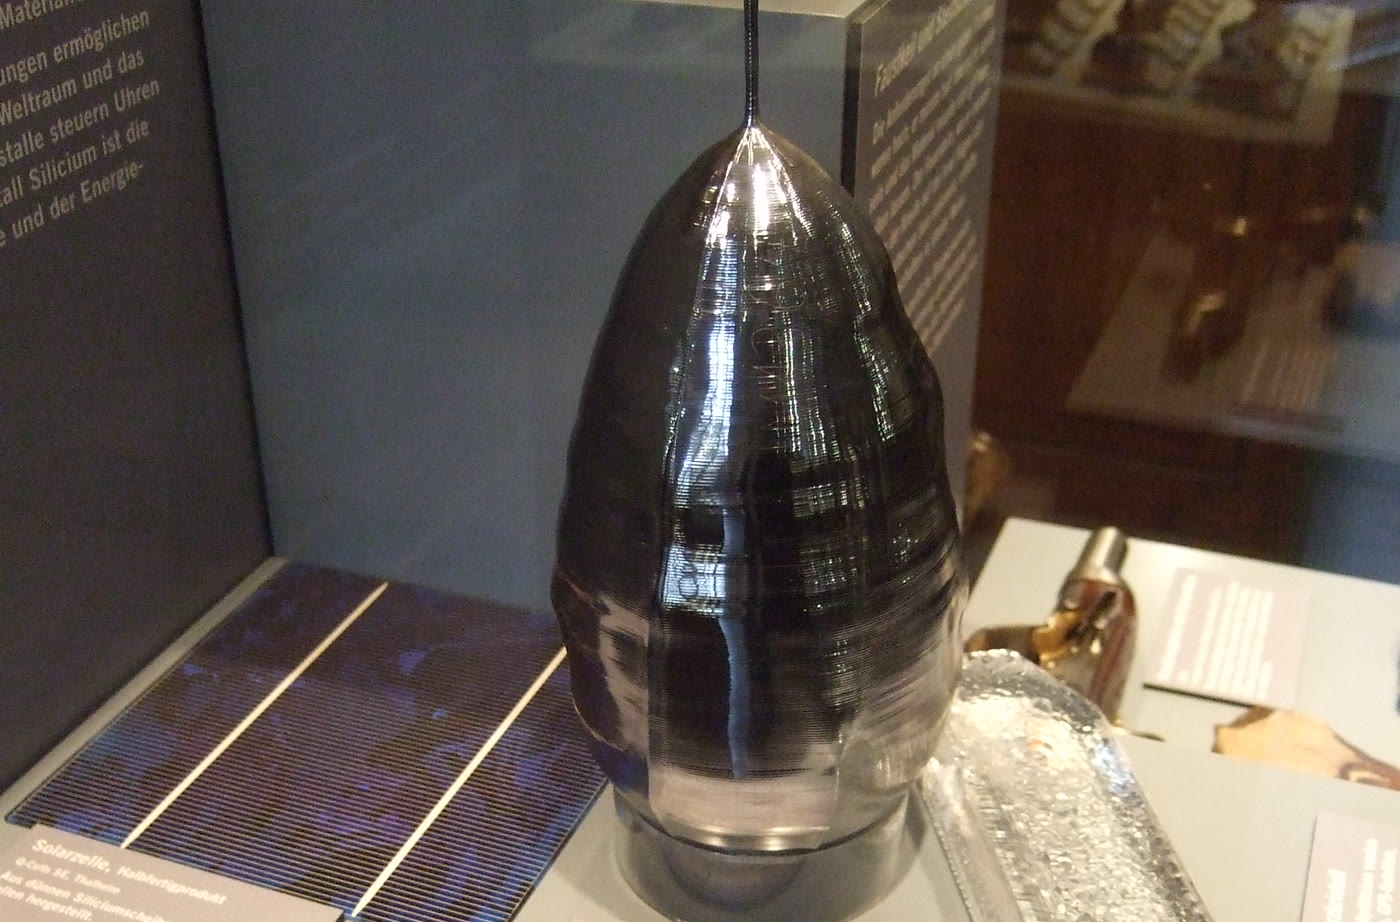
\includegraphics[width=0.5\linewidth]{images/book4/silicon-boule.jpg}

{\small بلورة أحادية من السيليكون مسحوبة من المصهور، معروضة بجانب خلية
شمسية مصنوعة من شريحة من مثل هذه البلورة. الصورة: سيباستيان فالروت،
ملكية عامة.}
\end{omfigure}

\begin{inthelab}[إنماء بلورة سيليكون]
في طريقة تشوخرالسكي، يُصهر سيليكون متعدد البلورات شديد النقاوة في
بوتقة من السيليكا تحت الأرغون، عند درجة أعلى قليلًا من درجة انصهاره، مع
إضافة \omterm{def:b3:solid-state:doping}{المطعِّم} إلى المصهور. وتُغمس بلورة بذرية صغيرة على قضيب دوّار في
المصهور وتُرفع ببطء: فيتبلور السيليكون عليها باتجاه
البذرة، وتحدد سرعة السحب والدوران القطر. ثم تُنشر السبيكة
إلى رقائق سمكها أقل من مليمتر. والسيلان وغازا التطعيم
الفوسفين والأرسين المستعملة في الخطوات اللاحقة ذاتية الاشتعال أو شديدة السمية،
ولا تُتداول إلا في منظومات صناعية محكمة الإغلاق.
\end{inthelab}

\section{العيوب النقطية}

\begin{definition}[العيوب النقطية]\label{def:b3:solid-state:defects}
\emph{العيب النقطي}\index{عيب نقطي} انحراف عن البلورة
المثالية متمركز في موقع واحد: فراغ، أو ذرة خلالية، أو ذرة
غريبة. وفي بلورة أيونية، \emph{عيب شوتكي}\index{عيب شوتكي}
زوج من الفراغات، فراغ كاتيوني وفراغ أنيوني، بعد أن ذهب الأيونان إلى
السطح؛ و\emph{عيب فرنكل}\index{عيب فرنكل} زوج مكوّن من
فراغ والأيون الذي غادره، جالسًا في موقع خلالي.
\end{definition}

\begin{omfigure}
\begin{tikzpicture}[scale=0.62]
  \begin{scope}
  \foreach \i in {0,...,5} \foreach \j in {0,...,4} {
    \pgfmathtruncatemacro{\pty}{mod(\i+\j,2)}
    \ifnum\pty=0 \fill[omDef!70] (\i,\j) circle (0.2); \else \fill[omThm!25] (\i,\j) circle (0.38); \draw[omThm!60] (\i,\j) circle (0.38); \fi
  }
  \fill[white] (2,2) circle (0.45); \draw[dashed] (2,2) circle (0.3);
  \fill[white] (3,2) circle (0.45); \draw[dashed] (3,2) circle (0.38);
  \node[font=\small\bfseries] at (2.5,5.0) {\foreignlanguage{arabic}{شوتكي \babelsublr{(NaCl)}}};
  \end{scope}
  \begin{scope}[xshift=8cm]
  \foreach \i in {0,...,5} \foreach \j in {0,...,4} {
    \pgfmathtruncatemacro{\pty}{mod(\i+\j,2)}
    \ifnum\pty=0 \fill[black!45] (\i,\j) circle (0.2); \else \fill[omMeth!25] (\i,\j) circle (0.38); \draw[omMeth!60] (\i,\j) circle (0.38); \fi
  }
  \fill[white] (2,2) circle (0.3); \draw[dashed] (2,2) circle (0.22);
  \fill[black!45] (2.5,2.5) circle (0.2);
  \draw[->, thick] (2.1,2.1) -- (2.38,2.38);
  \node[font=\small\bfseries] at (2.5,5.0) {\foreignlanguage{arabic}{فرنكل \babelsublr{(AgCl)}}};
  \end{scope}
\end{tikzpicture}

{\small \omterm{def:b3:solid-state:defects}{عيوب نقطية} في طبقة من بلورة من نمط ملح الطعام (نقاط صغيرة: كاتيونات؛
دوائر كبيرة: أنيونات؛ متقطع: فراغات). يسارًا: زوج شوتكي، كاتيون
وأنيون مفقودان. يمينًا: زوج فرنكل، أيون فضة انتقل من موقعه
إلى موضع خلالي.}
\end{omfigure}

\begin{theorem}[تركيز التوازن لعيوب شوتكي]\label{thm:b3:solid-state:schottky}
في بلورة MX من $N$ وحدة صيغية، يكون عدد أزواج شوتكي $n$ عند
التوازن، مع أنتالبي تكوين $\Delta H_S$ لكل زوج و$n \ll N$،
\[
  \frac{n}{N} = \eu^{-\Delta H_S/2kT}.
\]
\end{theorem}

\begin{proof}
يكلّف إنشاء $n$ زوجًا $n\,\Delta H_S$ ويعطي إنتروبيا تشكيلية، من
الطرق $\binom{N}{n}$ لاختيار الفراغات الكاتيونية ومثلها للأنيونات:
$S = 2k\ln\frac{N!}{n!(N - n)!}$. وبصيغة ستيرلينغ $\ln x! \approx x\ln x - x$،
\[
  G(n) = n\,\Delta H_S - 2kT\bigl[N\ln N - n\ln n - (N - n)\ln(N - n)\bigr].
\]
عند التوازن $\dd G/\dd n = 0$: $\Delta H_S - 2kT\ln\frac{N - n}{n} = 0$، ومنه $n/(N - n) = \eu^{-\Delta H_S/2kT}$، و$n/N$ من أجل
$n \ll N$. والإنتروبيا الاهتزازية للعيوب، المهملة هنا، تضرب
النتيجة في عامل ثابت.
\end{proof}

\begin{proposition}[عيوب فرنكل]\label{prop:b3:solid-state:frenkel}
مع $N$ أيونًا من النوع المتحرك، و$N_i$ موقعًا خلاليًا متاحًا لها 
و$\Delta H_F$ أنتالبي تكوين الزوج، يكون عدد أزواج فرنكل $n =
\sqrt{NN_i}\,\eu^{-\Delta H_F/2kT}$ (من أجل $n \ll N, N_i$).
\end{proposition}

\begin{proof}
الإنتروبيا الآن $S = k\ln\binom{N}{n} + k\ln\binom{N_i}{n}$، والتصغير نفسه يعطي
\[
  \Delta H_F = kT\ln\frac{(N - n)(N_i - n)}{n^2} \approx kT\ln\frac{NN_i}{n^2},
\]
ومنه النتيجة.
\end{proof}

يبيّن الجذر التربيعي أن العيوب تتكوّن أزواجًا: فكما في $n_i$ في \omterm{def:b3:solid-state:classes}{شبه الموصل}،
يحوي أُسّ تركيزها نصف طاقة التكوين. وتكوّن هاليدات
القلويات أساسًا \omterm{def:b3:solid-state:defects}{عيوب شوتكي}؛ أما هاليدات الفضة، التي يتسع أيونها الصغير القابل للاستقطاب
$\ce{Ag+}$ بين الأنيونات، فتكوّن أساسًا \omterm{def:b3:solid-state:defects}{عيوب فرنكل}.

\begin{definition}[ترميز كروغر--فينك]\label{def:b3:solid-state:kroger-vink}
\emph{ترميز كروغر--فينك}\index{ترميز كروغر--فينك} يكتب \omterm{def:b3:solid-state:defects}{العيب النقطي}
في الصورة $\mathrm{A_S^c}$: حيث A النوع الموجود في الموقع (V للفراغ، و$i$ موقعًا
للخلالي)، وS الموقع الذي يشغله في البلورة المثالية، وc شحنته
نسبةً إلى ذلك الموقع: $\bullet$ لكل وحدة موجبة، و$'$ لكل وحدة
سالبة، و$\times$ للصفر.
\end{definition}

وهكذا فإن $\mathrm{V_{Na}'}$ فراغ صوديوم (فالشحنة $+1$ المفقودة تترك شحنة نسبية $-1$)،
و$\mathrm{V_{Cl}^{\bullet}}$ فراغ كلوريد، و$\mathrm{Ag_i^{\bullet}}$ أيون فضة خلالي، و$\mathrm{Ca_{Na}^{\bullet}}$ أيون كالسيوم في
موقع صوديوم، و$\mathrm{O_O^{\times}}$ أيون أكسيد في موضعه. وتوازن شوتكي في NaCl هو
$\text{لا شيء} \rightleftharpoons \mathrm{V_{Na}' + V_{Cl}^{\bullet}}$، وتوازن فرنكل في AgCl هو
$\mathrm{Ag_{Ag}^{\times}} \rightleftharpoons \mathrm{Ag_i^{\bullet} + V_{Ag}'}$.

\begin{method}[كتابة معادلة عيوب]\label{met:b3:solid-state:kroger-vink}
\begin{enumerate}
  \item اكتب ما يضاف إلى البلورة المضيفة والعيوب التي يُحدثها.
  \item حصيلة المواقع: تُحفظ نسبة المواقع الكاتيونية إلى الأنيونية في البلورة المضيفة
        (والفراغات تُعدّ مواقع).
  \item حصيلة المادة: الذرات نفسها في الطرفين (فالفراغات لا كتلة لها؛
        وكذلك الإلكترونات $e'$ \omterm{def:b3:solid-state:carriers}{والثقوب} $h^\bullet$).
  \item حصيلة الشحنة: مجموعا الشحنات الفعالة متساويان.
\end{enumerate}
\end{method}

\begin{example}[الإيتريا في الزركونيا]
إذابة $\ce{Y2O3}$ في $\ce{ZrO2}$ تضع أيوني $\ce{Y^3+}$ في موقعي $\ce{Zr^4+}$، لكل منهما شحنة نسبية $-1$، 
وثلاثة أيونات أكسيد في مواقع الأكسجين؛ ونسبة البلورة المضيفة، كاتيون واحد لكل موقعي
أكسجين، تقتضي أربعة مواقع أكسجين للكاتيونين، فيبقى أحدها فارغًا:
\[
  \ce{Y2O3} \xrightarrow{\ce{ZrO2}} \mathrm{2\,Y_{Zr}' + 3\,O_O^{\times} + V_O^{\bullet\bullet}}.
\]
المواقع: 2 كاتيونيان، و4 للأكسجين؛ المادة: 2 Y و3 O؛ الشحنة: $2(-1) + 2 = 0$. فراغ أكسيد
واحد لكل أيوني إيتريوم: وهذا ما يجعل الزركونيا المثبَّتة بالإيتريا
موصلًا لأيونات الأكسيد.
\end{example}

\begin{definition}[مركز اللون]\label{def:b3:solid-state:colour-centre}
\emph{مركز اللون}\index{مركز اللون} \omterm{def:b3:solid-state:defects}{عيب نقطي} يمتص
الضوء المرئي، مثل إلكترون محتجز في فراغ أنيوني في هاليد
قلوي (مركز F)، فيلوّن بلورة شفافة لولاه.
\end{definition}

تسخين كلوريد الصوديوم في بخار الصوديوم أو تشعيعه يكوّن مراكز F: فيسلك
الإلكترون المحتجز سلوك \omterm{def:b3:quantum-model-systems:box}{جسيم في صندوق} بحجم الفراغ، 
ويمتص في المرئي، فتصير البلورة صفراء مائلة إلى البني.

\section{اللاتكافؤ الستوكيومتري}

\begin{definition}[المركبات غير الستوكيومترية]\label{def:b3:solid-state:non-stoichiometric}
\emph{المركب غير الستوكيومتري}\index{مركب غير ستوكيومتري}
صلب يتغير تركيبه على مجال حول نسبة بسيطة بين أعداد
صحيحة، وتستوعب \omterm{def:b3:solid-state:defects}{العيوب النقطية} الفرق.
\end{definition}

أكسيد الحديد(II) ليس أبدًا $\ce{FeO}$ بالضبط: فهو دائمًا ناقص الحديد،
$\mathrm{Fe_{1-x}O}$، حيث تحدد $x$ درجة الحرارة وضغط الأكسجين اللذان صُنع عندهما. ويُعوَّض كل $\ce{Fe^2+}$ مفقود باثنين من
$\ce{Fe^3+}$، وهما بلغة العيوب \omterm{def:b3:solid-state:carriers}{ثقبان} على مواقع الحديد.

\begin{proposition}[الناقلية وضغط الأكسجين]\label{prop:b3:solid-state:brouwer}
من أجل أكسيد ناقص الفلز $\mathrm{M_{1-x}O}$ عيوبه فراغات فلزية مشحونة شحنة مضاعفة
يعوّضها \omterm{def:b3:solid-state:carriers}{ثقوب}، يتغير تركيز \omterm{def:b3:solid-state:carriers}{الثقوب}، والناقلية، وفق
$p(\ce{O2})^{1/6}$. ومن أجل أكسيد ناقص الأكسجين يعوّضه إلكترونات، يتغيران وفق
$p(\ce{O2})^{-1/6}$.
\end{proposition}

\begin{proof}
يُنشئ أخذ الأكسجين فراغات فلزية:
\[
  \tfrac12\ce{O2} \rightleftharpoons \mathrm{O_O^{\times} + V_M'' + 2\,h^{\bullet}}, \qquad K = \frac{[\mathrm{V_M''}][\mathrm h^\bullet]^2}{p(\ce{O2})^{1/2}}
\]
(ونشاطية $\mathrm{O_O^{\times}}$ تساوي 1). 
وحصيلة الشحنة هي $[\mathrm h^\bullet] = 2[\mathrm{V_M''}]$، ومنه $[\mathrm h^\bullet]^3 = 2K\,p(\ce{O2})^{1/2}$ و$[\mathrm h^\bullet] \propto p(\ce{O2})^{1/6}$. ومن أجل
الحالة الناقصة الأكسجين، $\mathrm{O_O^{\times}} \rightleftharpoons \tfrac12\ce{O2} + \mathrm{V_O^{\bullet\bullet} + 2\,e'}$، $[\mathrm e'] = 2[\mathrm{V_O^{\bullet\bullet}}]$، والخطوات نفسها تعطي $[\mathrm e'] \propto p(\ce{O2})^{-1/6}$.
والناقلية متناسبة مع تركيز الحاملات.
\end{proof}

فمنحنى $\log\sigma$ بدلالة $\log p(\ce{O2})$ يخبر إذن بالعيوب الغالبة: فميله،
$\pm 1/4$ أو $\pm 1/6$، يتوقف على شحناتها.

\section{الموصلات الأيونية}

\begin{definition}[الموصلات الأيونية]\label{def:b3:solid-state:ionic-conductor}
\emph{الموصل الأيوني}\index{موصل أيوني} صلب يحمل التيارَ فيه
أيوناتٌ تتحرك عبر الشبكة. و\emph{الإلكتروليت
الصلب}\index{إلكتروليت صلب} موصل أيوني ناقليته الإلكترونية
مهملة، بحيث يستطيع أن يفصل بين قطبي
خلية كهركيميائية.
\end{definition}

\begin{proposition}[قانون أرينيوس للتوصيل الأيوني]\label{prop:b3:solid-state:ionic-arrhenius}
من أجل أيونات تتحرك بالقفز بين مواقع متجاورة فوق حاجز $E_a$،
$\sigma T = A\,\eu^{-E_a/kT}$.
\end{proposition}

\begin{proof}[برهان جزئي]
يحاول الأيون القفز بتواتر $\nu_0$ وينجح باحتمال $\eu^{-E_a/kT}$،
فيكون معامل انتشاره $D = \tfrac16\nu_0 z a^2\eu^{-E_a/kT}$ من أجل $z$ موقعًا مجاورًا على
مسافة $a$ (مشي عشوائي). وعلاقة نرنست--أينشتاين $\sigma = nq^2D/kT$ (نقبلها)، من أجل $n$
أيونًا متحركًا شحنته $q$ في وحدة الحجم، تعطي $\sigma T = (nq^2\nu_0za^2/6k)\,\eu^{-E_a/kT}$. 
والتركيز $n$ يحدده التطعيم في موصل خارجي المنشأ؛ وحين يكون
هو نفسه متكوّنًا حراريًا، تحوي $E_a$ أيضًا نصف أنتالبي التكوين.
\end{proof}

% ledger: trans:AgI
ثلاثة إلكتروليتات صلبة تبيّن المدى. ففي الزركونيا المثبَّتة بالإيتريا تتيح
فراغات الأكسيد التي يُحدثها \omterm{def:b3:solid-state:doping}{المطعِّم} لأيونات $\ce{O^2-}$ أن تقفز؛ ولا توصل توصيلًا مفيدًا
إلا ساخنة، عند عدة مئات من الدرجات المئوية. وفي ألومينا $\beta$، تتحرك أيونات الصوديوم في
مستويات مرصوصة رصًا رخوًا بين كتل الإسبينل، وهي أساس بطاريات الصوديوم--الكبريت.
ويصير يوديد الفضة موصلًا فائق الأيونية فوق \qty{146}{\celsius}،
حيث تتوزع أيونات الفضة فيه على مواقع أكثر بكثير من عدد الأيونات،
كأنها سائل تقريبًا داخل شبكة يوديد صلبة. وموصلات أيونات الليثيوم
(غارنيتات زركونات الليثيوم واللانثانوم، والكبريتيدات) هي إلكتروليتات
البطاريات الصلبة كليًا التي يجري تطويرها الآن.

\begin{omfigure}
\begin{tikzpicture}[font=\small, >=Stealth]
  \fill[omProp!25] (0,0) rectangle (2.4,3.2);
  \node[font=\scriptsize, align=center] at (1.2,0.6) {$\ce{ZrO2}$--$\ce{Y2O3}$\\ \foreignlanguage{arabic}{إلكتروليت صلب}};
  \draw[black!60, line width=2.5pt] (-0.07,0) -- (-0.07,3.2);
  \draw[black!60, line width=2.5pt] (2.47,0) -- (2.47,3.2);
  \node[font=\scriptsize, align=center] at (-2.0,1.4) {\foreignlanguage{arabic}{غاز العادم}\\ \foreignlanguage{arabic}{$p(\ce{O2})$ منخفض}};
  \node[font=\scriptsize, align=center] at (4.4,1.4) {\foreignlanguage{arabic}{هواء مرجعي}\\ $p(\ce{O2}) = \qty{0.21}{bar}$};
  \node[font=\scriptsize, anchor=north] at (-0.07,-0.05) {Pt};
  \node[font=\scriptsize, anchor=north] at (2.47,-0.05) {Pt};
  \draw[->, thick, omThm] (2.0,1.9) -- (0.4,1.9) node[midway, above, font=\scriptsize] {$\ce{O^2-}$};
  \node[font=\scriptsize, anchor=west] at (2.65,2.75) {$\ce{O2 + 4e- -> 2O^2-}$};
  \node[font=\scriptsize, anchor=east] at (-0.25,2.75) {$\ce{2O^2- -> O2 + 4e-}$};
  \draw (-0.07,3.2) -- (-0.07,4.0) -- (0.85,4.0);
  \draw (2.47,3.2) -- (2.47,4.0) -- (1.55,4.0);
  \draw (1.2,4.0) circle (0.35) node {V};
\end{tikzpicture}

{\small مقطع عرضي في مستشعر الأكسجين من الزركونيا: قطبان مساميان من البلاتين
على وجهي \omterm{def:b3:solid-state:ionic-conductor}{الإلكتروليت الصلب}، أحدهما في العادم والآخر في الهواء.
تحمل أيونات الأكسيد التيار عبر الإلكتروليت؛ ويقيس الجهد
النسبة بين ضغطي الأكسجين.}
\end{omfigure}

\begin{history}[الترانزستور والبلورة المسحوبة]
في سنة 1947 صنع جون باردين ووالتر براتين، في مجموعة ويليام شوكلي في مختبرات
بل، أول ترانزستور من بلورة جرمانيوم؛ وتقاسم الثلاثة
جائزة نوبل في الفيزياء لسنة 1956. وجاءت البلورات من طريقة وجدها يان
تشوخرالسكي سنة 1916 وهو يقيس سرعة تبلور الفلزات،
بسحب خيط من القصدير من المصهور: وهي، بعد تكييفها للجرمانيوم ثم للسيليكون،
لا تزال تصنع رقائق كل الدارات المتكاملة تقريبًا.
\end{history}

\section{تمارين}

\begin{exercise}[$\star$]\label{exo:b3:solid-state:1}
أعطِ مستويات هوكل الستة لسلسلة من ست ذرات بوحدة $|\beta|$، 
وعرض المجال الذي تمتد عليه.
\end{exercise}

\begin{exercise}[$\star$]\label{exo:b3:solid-state:2}
كم إلكترونًا تتسع له حزمة مبنية من المدارات s لعدد $N$ من الذرات؟ ولماذا
يكون الصوديوم والمغنيزيوم كلاهما فلزين؟
\end{exercise}

\begin{exercise}[$\star$]\label{exo:b3:solid-state:3}
قدّر طول موجة الضوء الذي تصدره صمامات ثنائية من فوسفيد الغاليوم
(\qty{2.26}{eV}) ونتريد الغاليوم (\qty{3.4}{eV})، باستعمال $\lambda \approx hc/E_g$.
\end{exercise}

\begin{exercise}[$\star$]\label{exo:b3:solid-state:4}
اكتب معادلات كروغر--فينك لإذابة $\ce{CaCl2}$ في $\ce{NaCl}$ و$\ce{Y2O3}$ في $\ce{ZrO2}$، 
وتحقّق من كل حصيلة.
\end{exercise}

\begin{exercise}[$\star\star$]\label{exo:b3:solid-state:5}
مع $N_c = \num{6.2e15}\,T^{3/2}$ و$N_v = \num{3.5e15}\,T^{3/2}$ (بوحدة $\unit{cm^{-3}}$) و$E_g = \qty{1.125}{eV}$ للسيليكون عند \qty{300}{K}،
و$N_c = \num{1.98e15}\,T^{3/2}$ و$N_v = \num{9.6e14}\,T^{3/2}$ و$E_g = \qty{0.661}{eV}$ للجرمانيوم، احسب $n_i$ لكل منهما، 
والنسبة بينهما.
\end{exercise}

\begin{exercise}[$\star\star$]\label{exo:b3:solid-state:6}
يُطعَّم السيليكون بالفوسفور بتركيز $\qty{1.0e16}{cm^{-3}}$. ومع $n_i = \qty{1.0e10}{cm^{-3}}$ عند \qty{300}{K}، أعطِ
تركيزي الإلكترونات \omterm{def:b3:solid-state:carriers}{والثقوب}.
\end{exercise}

\begin{exercise}[$\star\star$]\label{exo:b3:solid-state:7}
من أجل بلورة \cref{exo:b3:solid-state:6}، كم يرتفع \omterm{def:b3:solid-state:fermi}{مستوى فيرمي} فوق المستوى
الذاتي؟
\end{exercise}

\begin{exercise}[$\star\star$]\label{exo:b3:solid-state:8}
أنتالبي تكوين زوج شوتكي في NaCl نحو \qty{2.3}{eV} (معطيات
التمرين). احسب نسبة المواقع الشاغرة عند \qty{800}{K}، وعدد
الأزواج في مول.
\end{exercise}

\begin{exercise}[$\star\star$]\label{exo:b3:solid-state:9}
لعيّنة من أكسيد الحديد(II) (بنية ملح الطعام، أربعة مواقع أكسجين في الخلية)
$a = \qty{430.0}{pm}$ وكثافة \qty{5.70}{g.cm^{-3}} (معطيات التمرين). بافتراض
أن مواقع الأكسجين ممتلئة، أوجد $x$ في $\mathrm{Fe_{1-x}O}$.
\end{exercise}

\begin{exercise}[$\star\star\star$]\label{exo:b3:solid-state:10}
لموصل أيونات الليثيوم $\sigma = \qty{1.0e-4}{S.cm^{-1}}$ عند \qty{300}{K}، و$\qty{7.8e-4}{S.cm^{-1}}$ عند \qty{350}{K} 
و$\qty{3.6e-3}{S.cm^{-1}}$ عند \qty{400}{K} (معطيات التمرين). أوجد طاقة تنشيطه.
\end{exercise}

\begin{exercise}[$\star\star\star$]\label{exo:b3:solid-state:11}
بيّن أنه في أكسيد عيوبه الغالبة فراغات فلزية مشحونة شحنة أحادية
$\mathrm{V_M'}$ تعوّضها \omterm{def:b3:solid-state:carriers}{ثقوب}، تتغير الناقلية وفق $p(\ce{O2})^{1/4}$.
\end{exercise}

\begin{exercise}[$\star\star\star$]\label{exo:b3:solid-state:12}
في AgCl أنتالبي تكوين زوج فرنكل نحو \qty{1.4}{eV}، وهناك
موقعان خلاليان لكل أيون فضة (معطيات التمرين). احسب نسبة
أيونات الفضة في المواقع الخلالية عند \qty{600}{K}.
\end{exercise}

\section{مسألة: مستشعر الأكسجين في أنبوب العادم}

\begin{problem}[{مسألة نهاية الأسبوع --- مستشعر الأكسجين في أنبوب العادم:
عيوب الزركونيا المثبَّتة بالإيتريا، وناقليتها الأيونية ودرجة حرارة
تشغيلها، وجهد نرنست للخلية، والتبدّل بين العادم الفقير 
والغني}]
\label{pb:b3:solid-state:1}
% ledger: const:R, const:F, const:kB, const:e, const:NA, air:O2
إلكتروليت المستشعر زركونيا فيها 8.0\,mol\,\% من $\ce{Y2O3}$، ذات بنية الفلوريت
بأربعة مواقع كاتيونية وثمانية مواقع أكسجين في كل خلية مكعبة، $a = \qty{514}{pm}$؛ ويفصل قرص
سمكه \qty{1.0}{mm} ومساحته \qty{0.20}{cm^2} العادمَ عن الهواء. 
وتتبع ناقليته $\sigma T = A\eu^{-E_a/kT}$ مع $E_a = \qty{1.0}{eV}$ و$\sigma = \qty{0.030}{S.cm^{-1}}$ عند \qty{800}{\celsius}. وللعادم
الفقير $p(\ce{O2}) = \qty{0.010}{bar}$، وللعادم الغني $p(\ce{O2}) = \qty{1.0e-20}{bar}$ (كلها معطيات المسألة).

\medskip\noindent\textbf{الجزء الأول --- الإلكتروليت.}
\begin{enumerate}
  \item اكتب معادلة كروغر--فينك لإذابة $\ce{Y2O3}$ في $\ce{ZrO2}$.
  \item تحقّق من حصائل المواقع والمادة والشحنة فيها.
  \item كم فراغ أكسيد يتكوّن لكل أيون إيتريوم؟
  \item اكتب التركيب في الصورة $\mathrm{Zr_{1-x}Y_xO_{2-x/2}}$ واحسب $x$.
  \item احسب نسبة مواقع الأكسجين الشاغرة.
  \item احسب عدد الفراغات في الخلية.
  \item احسب تركيز الفراغات بوحدة $\unit{cm^{-3}}$.
\end{enumerate}

\medskip\noindent\textbf{الجزء الثاني --- الناقلية ودرجة الحرارة.}
\begin{enumerate}[resume]
  \item لماذا ترتفع الناقلية بحدة مع درجة الحرارة؟
  \item احسب $A$.
  \item احسب $\sigma$ عند \qty{700}{\celsius}.
  \item احسب $\sigma$ عند \qty{300}{\celsius}.
  \item احسب مقاومة القرص عند هاتين الدرجتين.
  \item تحتاج الإلكترونيات إلى مقاومة أدنى من \qty{1}{k\ohm}: أوجد أدنى درجة حرارة
        للتشغيل.
  \item لماذا تُزوَّد هذه المستشعرات بسخّان؟
\end{enumerate}

\medskip\noindent\textbf{الجزء الثالث --- جهد نرنست.}
\begin{enumerate}[resume]
  \item اكتب تفاعل القطب في جانب الهواء، بالترميز العادي
        وفي \omterm{def:b3:solid-state:kroger-vink}{ترميز كروغر--فينك}.
  \item بيّن أن جهد الخلية $E = (RT/4F)\ln\bigl(p_{\mathrm{air}}/p_{\mathrm{exh}}\bigr)$.
  \item احسب $RT/4F$ عند \qty{700}{\celsius}.
  \item ما الجهد لو كان العادم يحوي هواءً؟
  \item احسب تغير الجهد لكل عامل عشرة في $p(\ce{O2})$.
\end{enumerate}

\medskip\noindent\textbf{الجزء الرابع --- الفقير والغني والتبدّل.}
\begin{enumerate}[resume]
  \item احسب الجهد في العادم الفقير عند \qty{700}{\celsius}.
  \item احسب الجهد في العادم الغني عند \qty{700}{\celsius}.
  \item لماذا يكون $p(\ce{O2})$ صغيرًا إلى هذا الحد في العادم الغني؟
  \item يتبدّل التحكم في المحرك عند \qty{0.45}{V}: ما ضغط الأكسجين الذي
        يوافق ذلك؟
  \item لماذا يقفز الجهد عند النسبة الستوكيومترية بين الهواء والوقود، وكيف
        يستعمله التحكم في المحرك؟
  \item اذكر النتيجة: جهد المستشعر في العادم الغني عند \qty{700}{\celsius}.
\end{enumerate}
\end{problem}
